
\documentclass[xcolor=dvipsnames]{beamer} % dvipsnames gives more built-in colors
\usepackage[utf8]{inputenc}
\usepackage[spanish]{babel}

\mode<presentation> {

\usetheme{CambridgeUS}

%\setbeamertemplate{footline} % To remove the footer line in all slides uncomment this line
\setbeamertemplate{footline}[page number] % To replace the footer line in all slides with a simple slide count uncomment this line

\setbeamertemplate{navigation symbols}{} % To remove the navigation symbols from

\definecolor{utfsmred}{HTML}{D60019}
\definecolor{utfsmyellow}{HTML}{F7AE00}
\definecolor{utfsmgreen}{HTML}{008452}
\definecolor{utfsmblue}{HTML}{004B85}


\newenvironment<>{rosa}[1][]{
  \setbeamercolor{block title example}{fg=white,bg=blue!75!black}%
  \begin{example}#2[#1]}{
  \end{example}
}



\usecolortheme[named=utfsmblue]{structure}
\setbeamercolor{titlelike}{parent=structure,fg=utfsmblue}
\setbeamercolor{frametitle}{fg=utfsmblue}

%\setbeamercolor{section in head/foot}{bg=Brown}
%\setbeamercolor{author in head/foot}{bg=Brown}
%\setbeamercolor{date in head/foot}{fg=Brown}

\setbeamercolor*{enumerate item}{fg=utfsmred}
\setbeamercolor*{enumerate subitem}{fg=utfsmred}
\setbeamercolor*{enumerate subsubitem}{fg=utfsmred}

\setbeamercolor*{itemize item}{fg=utfsmred}
\setbeamercolor*{itemize subitem}{fg=utfsmred}
\setbeamercolor*{itemize subsubitem}{fg=utfsmred}

\setbeamercolor{item projected}{bg=utfsmred}


\setbeamertemplate{itemize items}[square]
\setbeamertemplate{enumerate items}[default]


\setbeamercolor{section in head/foot}{bg=utfsmblue}

\setbeamercolor{block title}{bg=utfsmblue!80,fg=white}
\setbeamercolor{block title alerted}{bg=utfsmred!80,fg=white}
\setbeamercolor{block title example}{bg=utfsmgreen!80,fg=white}

\setbeamertemplate{sections/subsections in toc}[square]
\setbeamercolor{section number projected}{bg=utfsmblue,fg=white}


}


\usepackage{graphicx} % Allows including images
\usepackage{booktabs} % Allows the use of \toprule, \midrule and \bottomrule in tables
\usepackage{listings}
\lstset{ %
language=C,
basicstyle=\normalsize\ttfamily,
keywordstyle=,
numbers=none,
numberstyle=\tiny\ttfamily,
stepnumber=1,
showspaces=false,
showstringspaces=false,
showtabs=false,
breaklines=true,
frame=tb,
framerule=0.5pt,
tabsize=4,
framexleftmargin=0.5em,
framexrightmargin=0.5em,
xleftmargin=0.5em,
xrightmargin=0.5em,
}

%----------------------------------------------------------------------------------------
%	TITLE PAGE
%----------------------------------------------------------------------------------------

\title{Permisos}
\subtitle{\small{Seminario de Desarrollo de Software - Casa Central.}}
\author{Maximiliano Osorio\\\small{mosorio@inf.utfsm.cl}} 
\institute[UTFSM]
{
Universidad Técnica Federico Santa María
\medskip
}
\date{\today} % Date, can be changed to a custom date

\begin{document}
	
%-=-=-=-=-=-=-=-=-=-=-=-=-=-=-=-=-=-=-=-=-=-=-=-=
%
%	TITLE PAGE
%
%-=-=-=-=-=-=-=-=-=-=-=-=-=-=-=-=-=-=-=-=-=-=-=-=








\maketitle

\begin{frame}[fragile]
    \frametitle{Usuarios}
    \begin{itemize}
    	\item Cada programa corre como un usuario particular.
    	\item Cada archivo es propiedad de un usuario.
    	\item Acceso a archivos y directorios están definidos por un usuario.
   		\item Los usuarios son cuentas asociadas a humanos o aplicaciones.
   		\item Identificados por UID 
    \end{itemize}
    \begin{lstlisting}
[mosorio@ssh ~]$ id
uid=5844(mosorio) gid=5844(mosorio) groups=5844(mosorio) context=unconfined_u:unconfined_r:unconfined_t:s0-s0:c0.c1023
    \end{lstlisting}
\end{frame}


\begin{frame}[fragile]
    \frametitle{Permisos y archivos}
    \begin{lstlisting}
[mosorio@ssh ~]$ ls -l
drwxr-xr-x   12 mosorio  staff       408 Apr  6 14:29 repos
-rw-r--r--    1 mosorio  staff        22 Mar 14 23:05 vtr
    \end{lstlisting}
\end{frame}

\begin{frame}[fragile]
    \frametitle{Permisos y procesos}
    \begin{lstlisting}[basicstyle=\tiny]
[mosorio@ssh ~]$ ps au
USER       PID %CPU %MEM    VSZ   RSS TTY      STAT START   TIME COMMAND
root      1726  0.0  0.0   4068   584 tty1     Ss+  Jan26   0:00 /sbin/mingetty
root      1729  0.0  0.0   4068   584 tty2     Ss+  Jan26   0:00 /sbin/mingetty
root      1731  0.0  0.0   4068   580 tty3     Ss+  Jan26   0:00 /sbin/mingetty
root      1733  0.0  0.0   4068   580 tty4     Ss+  Jan26   0:00 /sbin/mingetty
root      1735  0.0  0.0   4068   580 tty5     Ss+  Jan26   0:00 /sbin/mingetty
root      1752  0.0  0.0   4068   584 tty6     Ss+  Jan26   0:00 /sbin/mingetty
mosorio  13000  1.4  0.3 108172  3692 pts/1    Ss   23:50   0:00 -bash
mosorio  13128  0.0  0.1 108352  1132 pts/1    R+   23:50   0:00 ps au
ydossow  13280  0.0  0.2 106696  2080 pts/0    Ss+  Mar08   0:01 -bash
    \end{lstlisting}
\end{frame}



\begin{frame}{/etc/passwd}
Existe un archivo que guarda la información de los usuarios:\textbf{/etc/passwd}
	\begin{enumerate}
\item Username: Nombre
\item Password placeholder
\item User ID (UID): Identificador único del usuario
\item Group ID (GID): Identificador único del grupo
\item User ID Info: Información extra del usuario, ej. nombre completo.
\item Home directory: Ruta absoluta del home del usuario.
\item 	Command/shell: Ruta absoluta del comando o shell (/bin/bash). 
	\end{enumerate}
	
	\begin{figure}
		\centering
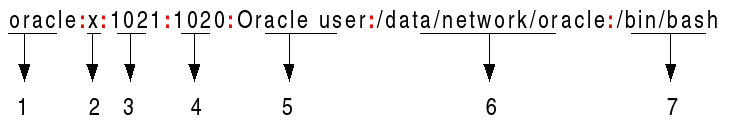
\includegraphics[width=\textwidth,height=0.8\textheight,keepaspectratio]{images/passwd}
\end{figure}
\end{frame}


\begin{frame}{UID}
	Los UID tienen un estandar:
	\begin{itemize}
		\item UID 0 (zero) es root.
		\item UID 1-99 están reservados para cuentas predefinas.
		\item UID 100-999 están reservadas para cuentas de sistemas.
	\end{itemize}
	
	Es común ver usuarios con shell \textbf{/sbin/nologin} para prevenir que no existan logeo.\\
%	Existe un pseduo-user \textit{nobody} con valor -1 o -2, son utilizados cuando se montan desde NFS cuando no hay confianza.
\end{frame}



%User ID (UID): Each user must be assigned a user ID (UID). UID 0 (zero) is reserved for root and UIDs 1-99 are reserved for other predefined accounts. Further UID 100-999 are reserved by system for administrative and system accounts/groups.

\begin{frame}{Grupos}
Como los usuarios, cada grupo tiene un nombre y id (GID), se definen en \textbf{/etc/group}
	\begin{itemize}
		\item Cada usuario tiene un \textbf{grupo primario}.
		\item La relación se puede encontrar en la tercera columna de /etc/passwd.
		\item Existen grupos extras que se encuentran en /etc/group.
		\item Un usuario siempre tiene un grupo, este grupo es llamado primario y tiene el mismo nombre.
	\end{itemize}
\end{frame}

%\begin{frame}{Grupos suplemtarios}
%En la última columna de \textbf{/etc/group} se pueden ver.
%	
%\end{frame}
%
%
%
%\begin{frame}{/etc/shadow}
%\begin{itemize}
%	\item Mantiene las passwords encriptadas.
%	\item shadow sólo puede ser leido por superuser.
%	\item /etc/shadow y /etc/passwd son independientes,  useradd con passwd mantiene a ambos
%\end{itemize}
%\end{frame}


\begin{frame}{/etc/shadow}

	\begin{figure}
		\centering
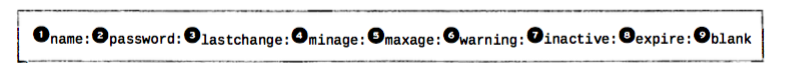
\includegraphics[width=\textwidth,height=0.8\textheight,keepaspectratio]{images/shadow}
\end{figure}


\begin{itemize}
	\item 1. login name.
	\item 2. Encrypted password.
	\item 3. Fecha del ultimo cambio de password.
	\item 4. Mínimos de número de días para que password pueda cambiar.
	\item 5. Máximo de número de días para la password deba ser cambia.
	\item 8. Fecha de expiración
\end{itemize}
\end{frame}






\begin{frame}[fragile]
    \frametitle{root user}
    Todos los sistemas tiene un usuario del tipo superuser
    \begin{itemize}
    	\item superuser: es un usuario que tiene poder supremo y total del sistema.
    	\item Con este gran privilegio viene una gran responsabilidad.
    \end{itemize}

%\begin{alertblock}{Warning}
%\begin{itemize}
%	\item No es recomendado entrar al sistema directamente con root.
%	\item Usar root solamente cuando sea necesario.
%	\item Lo recomendando es entrar como un usuario sin privilegios y luego obtenerlos (su, sudo, PolicyKit).
%	\item Tener un entorno grafico conlleva tener mayor posibilidad de vulnerabilidades.
%\end{itemize}
%\end{alertblock}

\end{frame}

\begin{frame}[fragile]
    \frametitle{su -}
    \begin{itemize}
    	\item El comando su permite cambiar a otra cuenta, si el usuario no se encuentra especificado en el comando, por defecto es root.
    	\item El comando \textbf{su username} inicia un shell con las configuraciones de ambientes del usuario que lanza el comando.
    	\item El comando \textbf{su - username} inicia un shell con las configuraciones de ambientes del usuario \textbf{username}    \end{itemize}
\begin{alertblock}{Warning}
\begin{itemize}
	\item Con \textit{su -} se puede suplantar a un usuario.
	\item Usar \textbf{/bin/su} es recomendado.
\end{itemize}
\end{alertblock}


\end{frame}


\begin{frame}[fragile]
    \frametitle{sudo}

\begin{itemize}
	\item \textbf{sudo} toma un argumento y lo ejecuta como root
	\item \textbf{sudo} con consulta a \textbf{/etc/sudoers} para conocer quien está autorizado.
	\item Cada cinco minutos preguntará la clave.
\end{itemize}    	
\end{frame}

\begin{frame}[fragile]
    \frametitle{sudo}
    
    \begin{itemize}
    	\item La desventaja de usar \textbf{su} es que la cuenta tiene todos los privilegios.
    	\item \textbf{sudo} permite acceder tareas de administración en base al archivo \textbf{/etc/sudoers} y se debe ingresar la \textit{password}.
    	\item Permite manejar con granularidad en los permisos.
    	\item Al utilizar sudo queda un log del comando
  
    \end{itemize}
    
     \begin{lstlisting}
[root@yanara ~]# tail -f /var/log/secure
Oct 14 16:09:45 yanara sudo: linets : TTY=pts/1 ; PWD=/home/linets ; USER=root ; COMMAND=/sbin/ip a
Oct 14 16:09:47 yanara sudo: linets : TTY=pts/1 ; PWD=/home/linets ; USER=root ; COMMAND=/bin/su -
Oct 14 16:09:47 yanara su: pam_unix(su-l:session): session opened for user root by linets(uid=0)
    \end{lstlisting}
\end{frame}




\begin{frame}[fragile]
\frametitle{sudo}
El usuario root puede ejecutar desde todas las terminales actuando como ALL (any) usuarios y correr ALL (any) comando.

    \begin{lstlisting}
    root ALL=(ALL) ALL

    \end{lstlisting}
    
\end{frame}


\begin{frame}[fragile]
\frametitle{sudo}
El usuario operator puede correr \textbf{power off} de cualquier terminal.
    \begin{lstlisting}
operator ALL= /sbin/poweroff

    \end{lstlisting}
    
\end{frame}


%\begin{frame}[fragile]
%\frametitle{sudo}
%
%    \begin{lstlisting}
%User_Alias OPERATORS = joe, mike, jude 
%Runas_Alias OP = root, operator 
%Host_Alias OFNET = 10.1.2.0/255.255.255.0 
%Cmnd_Alias PRINTING = /usr/sbin/lpc, /usr/bin/lprm
%OPERATORS ALL=ALL
%linus ALL=(OP) ALL
%user2 OFNET=(ALL) ALL
%user3 ALL= PRINTING
%
%    \end{lstlisting}
%    
%\end{frame}



\begin{frame}[fragile]
    \frametitle{Manejando cuentas locales}


% Please add the following required packages to your document preamble:
% \usepackage{graphicx}
\begin{table}[]
\centering

\resizebox{\textwidth}{!}{%
\begin{tabular}{|l|l|}
\hline
Utilities & Description \\ \hline
id & Displays user and group IDs. \\ \hline
useradd, usermod, userdel & \begin{tabular}[c]{@{}l@{}}Standard utilities for adding, \\ modifying, and deleting user accounts.\end{tabular} \\ \hline
\begin{tabular}[c]{@{}l@{}}groupadd, groupmod, \\ groupdel\end{tabular} & \begin{tabular}[c]{@{}l@{}}Standard utilities for adding, \\ modifying, and deleting groups.\end{tabular} \\ \hline
gpasswd & \begin{tabular}[c]{@{}l@{}}Standard utility for administering \\ the /etc/group configuration file.\end{tabular} \\ \hline
\end{tabular}
}
\end{table}
Para conocer más de los comandos asociados, se recomienda consultar
\href{https://access.redhat.com/documentation/en-US/Red_Hat_Enterprise_Linux/7-Beta/html/System_Administrators_Guide/s1-users-tools.html#s2-users-tools-users-add}{RHEL Doc: Crear, eliminar y manejo de grupos}
\end{frame}



\begin{frame}[fragile]
    \frametitle{useradd}
Crear una usuario y setea los campos en \textbf{/etc/password}. No setea una password

    \begin{lstlisting}
useradd mosorio
    \end{lstlisting}
\end{frame}




%\begin{frame}[fragile]
%    \frametitle{usermod}
%Modifica la cuenta del usuario
%	\begin{figure}
%		\centering
%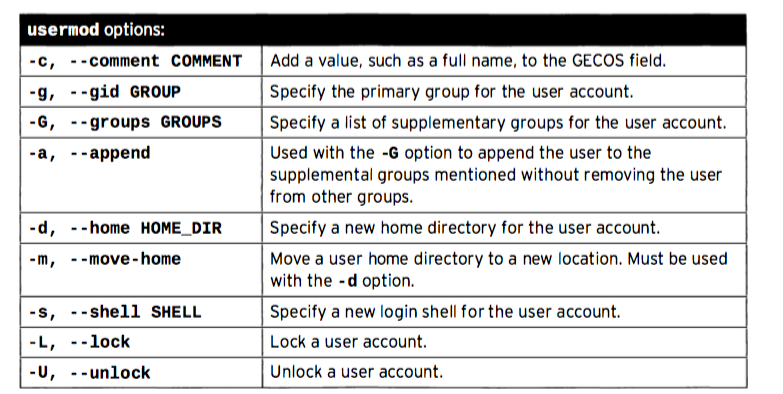
\includegraphics[width=\textwidth,height=0.8\textheight,keepaspectratio]{images/usermod}
%\end{figure}
%\end{frame}


\begin{frame}[fragile]
    \frametitle{userdel}

\begin{itemize}
	\item \textbf{userdel username} remueve al usuario pero deja el home intacto.
	\item \textbf{userdel -r username} y el home.
	\begin{alertblock}{userdel}
	Cuando un usuario es eliminado sin la opción -r, el sistema deja los archivos con UID no asignado.	
	\end{alertblock}

\end{itemize}

\end{frame}

\begin{frame}[fragile]
    \frametitle{leak}
	\begin{figure}
		\centering
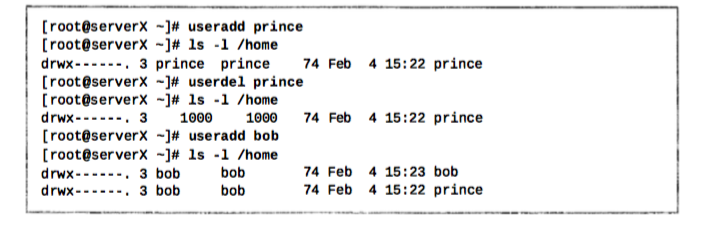
\includegraphics[width=\textwidth,height=0.8\textheight,keepaspectratio]{images/leak}	\end{figure}
	\begin{lstlisting}
		find / -nouser -o nogroup 2> /dev/null
	\end{lstlisting}
\end{frame}




\begin{frame}[fragile]
    \frametitle{Quitando acceso}

	\begin{lstlisting}
[mosorio@ip122 ~]$ sudo usermod -L vonbrand
[mosorio@ip122 ~]$ su - vonbrand
Password:
su: Authentication failure
	\end{lstlisting}
\end{frame}




\begin{frame}[fragile]
    \frametitle{Linux file system permissions}
    El acceso a los archivos son controlados por Linux.
    \begin{itemize}
    	\item Grupos de permisos:
        \begin{itemize}
    	\item El archivo tiene un dueño.
    	\item El archivo tiene un grupo.
    	\item Se puede definir permisos para el dueño, grupo y todos los demás usuarios.
    	\end{itemize}
    	\item Tipos permisos:
        \begin{itemize}
    	\item read: Permite leer el archivo
    	\item write: Permite escribir o modificar el archivo.
    	\item execute: Permite ejecutar el archivo o ver los contenidos de un directorio.
    	\end{itemize}
    	
   	\end{itemize}
   	\begin{alertblock}{Precedencia}
   	
   	Existe precedencia, primero se ve owner, después group y luego others.	
   	\end{alertblock}

\end{frame}

\begin{frame}[fragile]
    \frametitle{Viendo los permisos}
    \begin{block}{Permisos}
    	\textbf{r:} read.
    	\textbf{w:} write.
    	\textbf{x:} execute.
    \end{block}
    \begin{lstlisting}
drwxrwxr-x.  2 mosorio mosorio  taller_redes
drwx------.  2 mosorio mosorio  Templates
drwxr-xr-x.  6 mosorio mosorio  term.js
-rw-rw-r--.  1 mosorio mosorio  testing
-rw-rw-r--.  1 mosorio mosorio  test.sh
drwxrwxr-x.  2 mosorio mosorio  tmp
-rw-rw-r--.  1 mosorio mosorio  Tor_ip_list
    \end{lstlisting}
\end{frame}


%\begin{frame}[fragile]
%    \frametitle{Ejercicio V/F}
%Usuarios y sus grupos
%    \begin{lstlisting}
%juana    juana,ricardo
%tulio   tulio,ricardo
%patana   patana,mario
%freddy    freddy,mario
%    \end{lstlisting}
%    \begin{lstlisting}
%drwxrwxr-x  tulio   ricardo dir
%-rw-rw-r--  juana   juana   lfile1
%-rw-r--rw-  juana   ricardo lfile2
%-rw-rw-r--  tulio   ricardo rfile1
%-rw-r--r--  tulio   ricardo rfile2
%    \end{lstlisting}
%\end{frame}
%
%\begin{frame}[fragile]
%    \frametitle{Ejercicio}
%
%    \begin{lstlisting}
%drwxrwxr-x  tulio   ricardo dir
%-rw-rw-r--  juana   juana   lfile1
%-rw-r--rw-  juana   ricardo lfile2
%-rw-rw-r--  tulio   ricardo lfile1
%-rw-r--r--  tulio   ricardo rfile2
%    \end{lstlisting}
%    
%\begin{itemize}
%    \item juana es la unica persona que pueden cambiar los contenidos de lfile1
%    \item tulio puede ver los contenidos lfile2 pero no puede modificar a lfile2
%    \item tulio puede borrar lfile1 y lfile2
%    \item patana puede cambiar los contenidos de lfile2
%    \item juana puede cambiar los contenidos de rfile1.
%\end{itemize}
%\end{frame}
%


\begin{frame}[fragile]
    \frametitle{Método simbolico}

    \begin{lstlisting}
chmod WhoWhatWhich file|directory
    \end{lstlisting}
    
    \begin{itemize}
    	\item who es u,g,o,a (user, group, other, all)
    	\item what es +,-,= (add, remove, exactly)
    	\item which es r,w,x (read, write, executable)
    \end{itemize}

\end{frame}

\begin{frame}[fragile]
    \frametitle{Método numerico}
Cada digito representa un nivel de acceso: user, group, other
    \begin{lstlisting}
chmod ### file|directory
    \end{lstlisting}
    \begin{itemize}
  	\item \# es la suma de r=4, w=2 y x=1.
    \end{itemize}

\end{frame}


\begin{frame}[fragile]
\begin{itemize}
	\item     \frametitle{Ejemplos}
Remueve los permisos de lectura y escritura para el grupo y otros sobre el file1
    \begin{lstlisting}
chmod go-rw file1
    \end{lstlisting}

\item Añade permisos de ejecución al archivo 2.
    \begin{lstlisting}
chmod a+x file2
    \end{lstlisting}
    
\item Setea permisos todos los permisos para el dueño, lectura y ejecución para el grupo y nada para otros.
    \begin{lstlisting}
chmod 750 sampledir
    \end{lstlisting}
    

\end{itemize}
\begin{block}{Recursividad}
chmod -R, permite cambiar los permisos recursivamente.	
    \end{block}
\end{frame}




\begin{frame}[fragile]
    \frametitle{Cambiando dueños}
Por defecto cuando se crea un archivo o directorio el dueño del éste, es quien ejecutó el comando.\\
Para cambiar el dueño se utiliza \textbf{chown}.

    \begin{lstlisting}
chown student folder
    \end{lstlisting}
    

    \begin{lstlisting}
chown student:student folder
    \end{lstlisting}


    \begin{lstlisting}
chown :student folder
    \end{lstlisting}
    
    \begin{lstlisting}
chown -R student:student folder
    \end{lstlisting}
    
    
\end{frame}


\begin{frame}[fragile]
    \frametitle{setuid}


\begin{itemize}
	\item setuid: significa que el \textbf{command} va correr como el dueño del archivo.
	\begin{lstlisting}
[mosorio@ssh ~]$ ls -l /usr/bin/passwd
-rwsr-xr-x. 1 root root 30768 Feb 17  2012 /usr/bin/passwd
	\end{lstlisting}
\end{itemize}    
\end{frame}

\begin{frame}[fragile]
    \frametitle{sticky}

\begin{itemize}
	\item sticky: se setea a un directorio y significa que solo el usuario dueño y root pueden borrar el archivo.
	\begin{lstlisting}
[mosorio@ssh ~]$ ls -ld /tmp/
drwxrwxrwt. 3 root root 4096 Oct 14 18:55 /tmp/

	\end{lstlisting}

\end{itemize}    
    
\end{frame}


\begin{frame}[fragile]
    \frametitle{setgid}
	\begin{itemize}
		\item En archivos: se ejecutan como el dueño.
		\item En directorios: los archivos nuevos en el directorio tienen de dueño al dueño del directorio.
	\end{itemize}

\end{frame}

\begin{frame}[fragile]
   \frametitle{setuid, setgid, sticky}

\begin{itemize}	\item Simbolicamente: u+s, g+s, o+t
	\item x: 4\#\#\#, 2\#\#\#, 1\#\#\#
\end{itemize}

\begin{lstlisting}
chmod g+s directory
chmod 2700 directory
\end{lstlisting}
\end{frame}

\begin{frame}[fragile]
    \frametitle{Procesos}
   \begin{itemize}
        	\item Todo proceso y archivos tiene un usuario relacionado.
    	\item El usuario está asociado al proceso y determina los archivos y directorios que son accesibles.
   \end{itemize}
\begin{lstlisting}[basicstyle=\tiny]
[mosorio@ssh ~]$ ps au
USER       PID %CPU %MEM    VSZ   RSS TTY      STAT START   TIME COMMAND
root      2091  0.0  0.0   4064   348 tty1     Ss+  Aug26   0:00 /sbin/mingetty /dev/tty1
root      2093  0.0  0.0   4064   348 tty2     Ss+  Aug26   0:00 /sbin/mingetty /dev/tty2
root      2095  0.0  0.0   4064   352 tty3     Ss+  Aug26   0:00 /sbin/mingetty /dev/tty3
root      2097  0.0  0.0   4064   348 tty4     Ss+  Aug26   0:00 /sbin/mingetty /dev/tty4
root      2099  0.0  0.0   4064   348 tty5     Ss+  Aug26   0:00 /sbin/mingetty /dev/tty5
root      2101  0.0  0.0   4064   348 tty6     Ss+  Aug26   0:00 /sbin/mingetty /dev/tty6
mosorio  26034  0.1  0.3 108156  3696 pts/2    Ss   20:22   0:00 -bash
mosorio  26238  0.0  0.1 108340  1108 pts/2    R+   20:24   0:00 ps au
ydossow  26794  0.0  0.1 106544  1920 pts/0    Ss   Oct09   0:00 -bash
ydossow  27246  0.0  0.3  60472  3864 pts/0    S+   Oct09   0:08 ssh root@fw
ydossow  28304  0.0  0.1 106544  1976 pts/1    Ss+  Oct09   0:00 -bash
    \end{lstlisting}
\end{frame}


%TODO: ¿HACER LAB?

\end{document}